\documentclass[a4paper,12pt]{article}
\usepackage{CJKutf8}
\usepackage{multirow}
\usepackage{graphicx}
\usepackage{amsmath}
\usepackage{amsfonts}
\usepackage{enumerate}
\usepackage{fancyhdr}
\usepackage{setspace}
\usepackage{bm}
%\pagestyle{fancy}
%\lhead{}
%\rhead{\bfseries Integral on lines and surfaces}
%\lfoot{Calculus}
%\cfoot{China University of Petroleum-Beijing}
%\rfoot{\thepage}
%\renewcommand{\headrulewidth}{0.4pt}
%\renewcommand{\footrulewidth}{0.4pt}
%%%% 段落首行缩进两个字 %%%%
\makeatletter
\let\@afterindentfalse\@afterindenttrue
\@afterindenttrue
\makeatother
\setlength{\parindent}{2em}  %中文缩进两个汉字位

\newcounter{solution}
\newcommand\TheSolution{%
  \textbf{Solution:}\\%
}

%%%% 下面的命令重定义页面边距,使其符合中文刊物习惯 %%%%
\addtolength{\topmargin}{-54pt}
\setlength{\oddsidemargin}{0.63cm}  % 3.17cm - 1 inch
\setlength{\evensidemargin}{\oddsidemargin}
\setlength{\textwidth}{14.66cm}
\setlength{\textheight}{24.00cm}    % 24.62

%%%% 下面的命令设置行间距与段落间距 %%%%
\linespread{1.4}
% \setlength{\parskip}{1ex}
\setlength{\parskip}{0.5\baselineskip}

%%%% 定理类环境的定义 %%%%
\newtheorem{example}{Example}             % 整体编号
\newtheorem{algorithm}{算法}
\newtheorem{theorem}{Theorem}[section]  % 按 section 编号
\newtheorem{definition}{Definition}
\newtheorem{axiom}{公理}
\newtheorem{property}{性质}
\newtheorem{proposition}{命题}
\newtheorem{lemma}{引理}
\newtheorem{corollary}{推论}
\newtheorem{remark}{注解}
\newtheorem{condition}{条件}
\newtheorem{conclusion}{结论}
\newtheorem{assumption}{假设}

%%%% 重定义 %%%%
\renewcommand{\contentsname}{目录}  % 将Contents改为目录
\renewcommand{\abstractname}{摘要}  % 将Abstract改为摘要
\renewcommand{\refname}{参考文献}   % 将References改为参考文献
\renewcommand{\indexname}{索引}
%\renewcommand{\figurename}{图}
\renewcommand{\tablename}{表}
\renewcommand{\appendixname}{附录}
\renewcommand{\algorithm}{算法}

\begin{document}
\begin{CJK}{UTF8}{gbsn}
\title{曲线,曲面积分}
\author{武国宁\footnote{电子邮件: wuguoning@163.com}\\[2ex]
 中国石油大学-北京\\[2ex]}
\date{2017年8月}
\maketitle

\section{第一类曲线曲面积分}
\subsection{第一类曲线积分}
    \subsubsection{第一类曲线积分定义}
\begin{definition}
    设$L$是空间$\mathbb{R}^3$上可求长的连续曲线,其端点为$A$和$B$,函数$f(x,y,z)$在
    $L$上有界。令$A = P_0, B = P_n$,在$L$上顺次的插入分点$P_1,P_2, \cdots, P_{n-1}$.
    分别在每个小弧段上任意取一点$\left(\xi_i,\eta_i,\zeta_i\right)$,
    并记第$i$个弧段$P_{i-1}P_i$的长度为$\Delta s_i(i=1,2,\cdots,n)$
    做和式
    \[
        \sum_{i=1}^{n}f(\xi_i,\eta_i,\zeta_i)\Delta s_i
    \]
    如果当所有小弧段的最长长度趋于零时,这个和的极限存在且唯一,与
    分点和点的取法无关,则称该极限值为$f(x,y,z)$在曲线$L$上的第一类曲线
    积分,记为:
    \[
        \int_{L} f(x,y,z)\,\mathrm{d}s
    \]
    即,
    \[
        \int_{L} f(x,y,z)\,\mathrm{d}s = \lim_{\lambda \to 0}\sum_{i=1}^{n}f(\xi_i,\eta_i,\zeta_i)\Delta s_i
    \]
    其中$f(x,y,z)$ 称为被积函数,$L$称为积分路径。
\end{definition}

    \subsubsection{第一类曲线积分性质}
    \begin{property}{\textbf{(线性)}}
        如果函数$f,g$在$L$上的第一类曲线积分存在,则对于任意常数$\alpha \in \mathbb{R},
        \beta \in \mathbb{R}$,有
        \[
            \int_L \left(\alpha f + \beta g\right)\, \mathrm{d}s = \alpha\int_L f \, \mathrm{d}x
            + \beta \int_L g \, \mathrm{d}s.
        \]
    \end{property}
    \begin{property}{\textbf{(路径可加性)}}
        设曲线$L = L_1 + L_2$,如果函数$f$在$L$上的第一类曲线积分存在,则
        函数$f$在$L_1$和$L_2$上的积分也存在,反之亦然。且有
        \[
            \int_L f \,\mathrm{d}s = \int_{L_1} f \, \mathrm{d}s + \int_{L_2} f \, \mathrm{d}s
            \]
    \end{property}
    \begin{theorem}
        设函数$f(x,y,z)$在$L$上连续,则它在$L$上的第一类曲线积分存在,且有
        \[
            \int_L f(x,y,z)\, \mathrm{d}s = 
            \int_{\alpha}^{\beta} f(x(t),y(t),z(t))\sqrt{{\dot{x(t)}}^2+{\dot{y(t)}}^2+{\dot{z(t)}}^2}\, \mathrm{d}t
            \]
    \end{theorem}

    \begin{example}
        计算$\displaystyle \int_L e^{\sqrt{x^2+y^2}}\,\mathrm{d}s$, 其中$L$ 为圆周
        $x^2+y^2=a^2$,直线$y=x$及$x$轴在第一象限围城图形的边界。
    \end{example}
    \begin{example}
        已知一条非均匀金属线$L$的方程为
        \[
            x = e^t\cos t, y = e^t\sin t, z = e^t, 0 \le t \le 1.
        \]
        它在每一点的线密度与该点到原点的距离成反比,而且在点$(1,0,1)$处的线密度为1,
        求它的质量。
    \end{example}

    \subsection{曲面的面积}
    \subsubsection{曲面面积的计算}
    设曲面$\Sigma$的方程为 
    \[
        x = x(u,v), y = y(u,v), z = z(u,v), (u,v) \in D 
    \]
    则
    \[
        \bm{r}(u,v) = x(u,v)\bm{i} + y(u,v)\bm{j} + z(u,v)\bm{k},
        \]
    相应的\textbf{Jacobi}矩阵
    \[
        \left( \begin{array}{cc} \frac{\partial x}{\partial u} & \frac{\partial x}{\partial v} \\
            \frac{\partial y}{\partial u} & \frac{\partial y}{\partial v} \\
            \frac{\partial z}{\partial u} & \frac{\partial z}{\partial v} 
        \end{array} \right)
    \]
    满秩,考虑$D$中的一个矩形微元$\sigma$,它的四个顶点为:
    \[
        P_1(u_0,v_0), P_2(u_0+\Delta u, v_0), P_3(u_0+\Delta u, v_0 + \Delta v), P_4(u_0, v_0+\Delta v)
        \]
    它被影射为:
    \[
        Q_1 = \bm{r}(u_0,v_0),
        Q_2 = \bm{r}(u_0+\Delta u, v_0),
        Q_3 = \bm{r}(u_0+\Delta u, v_0 + \Delta v),
        Q_4 = \bm{r}(u_0+\Delta u, v_0 + \Delta v).
        \]

    那么有:
    \[
        \overrightarrow{Q_1Q_2} = \bm{r}(u_0+\Delta u, v_0) - \bm{r}(u_0,v_0)
                              = \bm{r}_u(u_0,v_0)\Delta u + \circ(\Delta u),
        \]
    \[
        \overrightarrow{Q_1Q_4} = \bm{r}(u_0, v_0+\Delta v) - \bm{r}(u_0,v_0)
                              = \bm{r}_v(u_0,v_0)\Delta v + \circ(\Delta v),
    \]
    \[
        \Delta S \approx \|\bm{r}_u(u_0,v_0) \times \bm{r}_v(u_0,v_0)\|\Delta u\Delta v.
    \]
    \[
        \mathrm{d}S = \|\bm{r}_u(u_0,v_0) \times \bm{r}_v(u_0,v_0)\|\Delta u\Delta v.
    \]
所以有,
\[
    \begin{split}
        S & = \iint_D \|\bm{r}_u(u_0,v_0) \times \bm{r}_v(u_0,v_0)\|\,\mathrm{d} u\mathrm{d} v \\
          & = \iint_D \sqrt{EG-F^2}\,\mathrm{d}u \mathrm{d}v.
    \end{split}
    \]
其中,
\[
    \sqrt{EG-F^2} = \|\bm{r}_u \times \bm{r}_v\| = \left[\frac{\partial(y,z)}{\partial(u,v)}\right]^2 + 
    \left[\frac{\partial(z,x)}{\partial(u,v)}\right]^2 + \left[\frac{\partial(x,y)}{\partial(u,v)}\right]^2 
    \]
现在考虑两种特殊情况:
\begin{enumerate}
    \item 设曲面的方程为$z = f(x,y), (x,y) \in D$ 其中$f(x,y)$ 为连续可微函数,
        $D$ 为具有分段光滑边界的有界区域。这是有:
        \[
            \bm{r} = x\bm{i} + y\bm{j} + z\bm{k}.
        \]
    这时有:
        \[
            EG - F^2 = \left(1+f_x^2\right)\left(1+f_y^2\right)-\left(f_xf_y\right)^2
            = 1+f_x^2+f_y^2.
        \]
    于是有,
        \[
            S = \iint_D \sqrt{1 + f_x^2(x,y) + f_y^2(x,y)}\, \mathrm{d}x\mathrm{d}y
        \]
\item 设曲面的方程为$H(x,y,z) = 0$,其中$H(x,y,z)$是连续可微函数,且在$\Sigma$
    上$H_z(x,y,z) \ne 0 $. 由隐函数存在条件有:$z = f(x,y), (x,y) \in D$
    从而有:
    \[
        \begin{split}
            S & = \iint_D \sqrt{1+f_x^2+f_y^2}\, \mathrm{d}x\mathrm{d}y \\
              & = \iint_D \sqrt{1+\left(-\frac{H_x}{H_y}\right)^2+\left(-\frac{H_y}{H_z}\right)^2}\, \mathrm{d}x\mathrm{d}y \\
              & = \iint_D \frac{\|grad H\|}{\left|H_z\right|}\,\mathrm{d}x\mathrm{d}y
        \end{split}
            \]
\end{enumerate}

\begin{example}
    求抛物面$z = x^2 + y^2$被平面$z = 1$所截出的部分的面积。
\end{example}
\begin{example}
    设$\Sigma$为球面$x^2+y^2+z^2 = 2Rz$包含在锥面$z^2 = 3\left(x^2+y^2\right)$内的部分,求它的面积。
\end{example}

\subsection{第一类曲面积分}
设空间中一曲面$\Sigma$上分布着质量,任意点$(x,y,z)$处的密度为$\rho(x,y,z)$,如何求
$\Sigma$的总质量。

\begin{definition}
    设曲面$\Sigma$为有界光滑(或分片光滑)曲面,函数$z = f(x,y,z)$在曲面$\Sigma$
    上有界。将曲面分成$n$片小的曲面$\Delta\Sigma_i,i=1,2,\cdots,n$,记$\Delta S_i$
    为第$i$块曲面的面积,在$\Delta\Sigma_i$上任取一点$(\xi_i,\eta_i,\zeta_i)$
    ,作和
    \[
        \sum_{i=1}^{n}f(\xi_i,\eta_i,\zeta_i)\Delta S_i
    \]
    如果当分割的细度趋于零时,这个和的极限存在且唯一,则称此极限为
    $f(x,y,z)$在曲面$\Sigma$上的第一类曲面积分,记为$\displaystyle \iint_{\Sigma} 
    f(x,y,z)\,\mathrm{d}S$.记为
    \[
        \iint_{\Sigma}f(x,y,z)\, \mathrm{d}S = \lim_{\lambda \to 0}
        \sum_{i=1}^{n}f(\xi_i,\eta_i,\zeta_i)\Delta S_i,
    \]
其中$\Sigma$为积分曲面,$f(x,y,z)$为被积函数。
\end{definition}
\subsubsection{第一类曲面积分的计算方法}
设$\Sigma$的方程为:
\[
    x = x(u,v), y = y(u,v), z = z(u,v), (u,v) \in D.
\]
$f(x,y,z)$在$\Sigma$上连续,则有:
\[
    \iint_{\Sigma}f(x,y,z)\, \mathrm{d}S = \iint_D f(x(u,v), y(u,v), z(u,v)
    \sqrt{EG-F^2}\, \mathrm{d}u \mathrm{d}v
\]
特别的,当曲面$\Sigma$的方程为$z = z(x,y), (x,y) \in D$,则有
\[
    \iint_{\Sigma}f(x,y,z)\, \mathrm{d}S = \iint_D f(x, y, z(x,y)
    \sqrt{1+z_x^2(x,y)+z_y^2(x,y)}\, \mathrm{d}x \mathrm{d}y
\]
\begin{example}
    计算$\displaystyle I = \iint_{\Sigma}\sqrt{\frac{x^2}{a^4} + \frac{y^2}{b^4} + \frac{z^2}{c^4}}\, \mathrm{d}S$
    其中,$\Sigma$为椭球面$\displaystyle \frac{x^2}{a^2} + \frac{y^2}{b^2} + \frac{z^2}{c^2} = 1, a,b,c>0.$
\end{example}


\section{第二类曲线,曲面积分}
\subsection{第二类曲线积分}
\subsubsection{Vector Fields}

Suppose a region in the plane or in the space is occupied by a moving 
fluid such as air or water. Imaging that the fluid is made up of a 
very large number of particles, and that any instant of time a particle 
has a velocity $\bm{v}$. If we take a picture of some particles at 
different position points at the same instant, we would expect to find 
that these velocities vary from position to position. We can think of a
velocity  vectors as being attached to each point of the fluid. Such a 
fluid exemplifies a \textbf{vector field.}
\graphicspath{
    {../Figs/}
}
\begin{figure}[htbp]
    \centering
    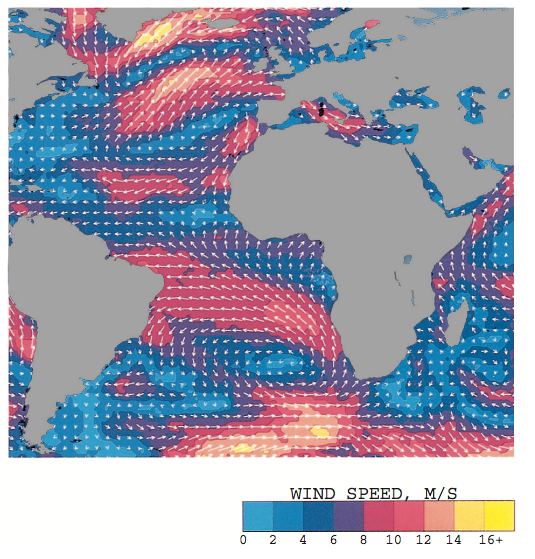
\includegraphics[width=0.7\textwidth]{vector.png}
    \caption{NASA's Seasat used radar to take 350,000 wind measurement 
    over the world's oceans. The arrows show wind direction; their length 
    and the color contouring indicate speed. Notice the heavy storm of Greenland.}
\end{figure}
Generally, a vector field on a domain in the plane or in space is a function 
that assigns a vector to each point in the domain. A field of three-dimensional 
vectors might have a formula like 
\[
    \bm{F}(x,y,z) = M(x,y,z)\bm{i} + N(x,y,z)\bm{j} + P(x,y,z)\bm{k}.
\]
\subsubsection{The Work of a Field}
Let $\bm{F}(x)$ be a continuous force field acting in a domain $G$ of 
the Euclidean space $\mathbb{R}^n$. The displacement of a test particle 
in the field is accompanied by work. We ask how we can compute the work
done by the field in moving a unit test particle along a given trajectory,
more precisely, a smooth path $\gamma: I(\gamma) \subset G $. It is know that in a 
constant field $\bm{F}$ the displacement by a vector $\bm{\xi}$
is associated with an amount of work $\langle \bm{F}, \bm{\xi}\rangle$ 

Suppose that the vector field 
\[
    \bm{F(t)} = M(x(t),y(t),z(t)\bm{i} + 
N(x(t),y(t),z(t))\bm{j} + P(x(t),y(t),z(t))\bm{k}
\]
represents a force throughout a region in space (it might be the force of 
gravity or an electromagnetic force of some kind), and $t \to \bm{r(t)}$ 
be a smooth mapping: $\gamma: I \to G$ defined on the closed interval 
$I = \left\{t \in \mathbb{R} | a \le t \le b\right\}$
\[
    \bm{r}(t) = x(t)\bm{i} + y(t)\bm{j} + z(t)\bm{k},
    a \le t \le b,
\]
is a smooth curve in the region.

We take a sufficiently fine partition of the closed interval $\left[a,b\right]$.
Then on each interval $\displaystyle I_i = \left\{t \in I | t_{i-1}\le t \le t_i \right\}$
of the partition we have the equality 
\[
    \Delta \bm{r}_i = \bm{r}_{i+1} - \bm{r}_i \approx 
    \dot{\bm{r}}(t_i)\Delta t_i = \left(\dot{x}(t_i),\dot{y}(t_i),\dot{z}(t_i)\right)\Delta t_i.
    \]
Since the field $\bm{F}(t)$ is continuous, it can be regarded a locally 
constant, and for that reason we can compute the work $\Delta A_i$ as 
\[
    \Delta A_i \approx \langle \bm{F}(t_i), \dot{\bm{r}}(t_i)\Delta t_i \rangle.
\]
\[
    A = \sum_{i}\Delta A_i \approx \sum_i \langle \bm{F}(t_i), \dot{\bm{r}}(t_i)\Delta t_i \rangle.
    \]
and so passing to the limit as the partition of the closed interval $I$ is 
refined, we find that 
\begin{equation}
    A = \int_a^b \langle \bm{F}(t), \dot{\bm{r}}(t) \rangle \, 
    \mathrm{d}t.
    \label{eq:eq1}
\end{equation}
The expression$\displaystyle \langle \bm{F}(t), \dot{\bm{r}}(t) \rangle
\mathrm{d}t$ is written as $\displaystyle \langle \bm{F}(t), \mathrm{d}\bm{r}
\rangle $, then as assume the coordinates in $\mathbb{R}^3$ are Cartesian 
coordinates, we can give this expression the form 
\[
    M\mathrm{d}x + N\mathrm{d}y + P\mathrm{d}z,
\]
after which we can writes Eq.~\ref{eq:eq1} as  
\begin{equation}
    A = \int_{\gamma}M\mathrm{d}x + N\mathrm{d}y + P\mathrm{d}z
    \label{eq:eq2}
\end{equation}
or as 
\begin{equation}
    A = \int_{\gamma}\omega_{\bm{F}}^1
    \label{eq:eq3}
\end{equation}

Formular~\ref{eq:eq3} provides the precise meaning of the integrals of the 
work 1-form along the path $\gamma$.

The expression of Equation~\ref{eq:eq2} can also be written as 
\begin{equation}
    A = \int_{\gamma}\bm{F}\cdot{\bm{T}}\,\mathrm{d}s
    \label{eq:eq4}
\end{equation}
where $\bm{T} = \left(\cos \alpha, \cos \beta, \cos \gamma\right)$ is the unit tangent 
vector.

\begin{example}
    Consider the force field $\displaystyle \bm{F} = \left(-\frac{y}{x^2 + y^2},
    \frac{x}{x^2 + y^2}\right)$ defined at all points of the plane $\mathbb{R}^2$ 
    except the origin. Let us compute the work of this field along the curve 
    $\gamma_1$ defined as $\displaystyle x = \cos t, y = \sin t, 0 \le t \le 2\pi$, and 
    along the curve defined by $\displaystyle x = 2 + \cos t, y = \sin t ,
    0 \le t \le 2\pi$
\end{example}

\begin{example}
    Let $\bm{r}$ be the radius vector of a point $(x,y,z) \in \mathbb{R}^3$
    and $r = \left|\bm{r}\right|$. Suppose a force field $\bm{F} = f(r)
    \bm{r}$ is defined everywhere in $\mathbb{R}^3$ except at the origin. 
    This is so-called central force field. Let up find the work of $\bm{F}$
    on a path: $\displaystyle \gamma: [0,1] \to \mathbb{R}^3 \setminus 0$
    \[
        \begin{split}
        \int_{\gamma}f(r)(x\mathrm{d}x + y\mathrm{d}y + z\mathrm{d}z) 
            & = \frac{1}{2}\int_{\gamma}f(r)\mathrm{d}(x^2+y^2+z^2)
            =\frac{1}{2}\int_0^1f(r(t))\,\mathrm{d}r^2(t) \\
            & = \frac{1}{2}\int_0^1f\left(\sqrt{u(t)}\right)\, \mathrm{d}u(t)
              = \frac{1}{2}\int_{r_0^2}^{r_1^2}f\left(\sqrt{u}\right)\, \mathrm{d}u \\
            & = \Phi(r_0,r_1).
        \end{split}
    \]
In particular, for the gravitational field $\displaystyle 
    \frac{1}{r^3}\bm{r}$ of a unit point mass located at 
    the origin, we obtain 
    \[
        \Phi(r_0,r_1) = \frac{1}{2} \int_{r_0^2}^{r_1^2}\frac{1}
        {u^{\frac{3}{2}}}\, \mathrm{d}u = \frac{1}{r_0} 
        - \frac{1}{r_1}
    \]
\end{example}
\begin{example}
    Find the work done by a variable force over a space curve, where 
    the force is $\bm{F} = (y-x^2)\bm{i} + (z-y^2)\bm{j} 
    + (x-z^2)\bm{k}$ over the curve $\bm{r}(t) = t\bm{i} + 
    t^2\bm{j}+t^3\bm{k}$, from $(0,0,0)$ to $(1,1,1)$.
\end{example}

\begin{example}
    Find flow along a helix: A fluid's velocity field is 
    $\displaystyle \bm{F} = x\bm{i} + z \bm{j} + k \bm{k} $.
    Find the flow along the helix $\bm{r}(t) = \cos t\bm{i} + 
    \sin t \bm{j} + t\bm{k}$
\end{example}

\subsubsection{Flux Across a Plane Curve}
To find the rate at which a fluid is entering or leaving a region enclosed
by a smooth curve $C$ in the xy-plane, we calculate the line integral over 
$C$ of $\bm{F}\cdot\bm{n}$, the scalar component of the fluid's velocity 
field in the direction of the curve's outward-pointing normal vector.
The value of this integral is the flux \footnote{Flux is a Latin word for flow,
but many flux calculation involve no motion at all.}
of $\bm{F}$ across $C$.

\begin{definition}
    If $C$ is a smooth curve in the domain of a continuous vector field 
    $\bm{F} = M(x,y)\bm{i} + N(x,y)\bm{j}$ in the plane and 
    if $\bm{n}$ is the outward-pointing unit normal vector on $C$, the 
    flux of $\bm{F}$ across $C$ is :
    \begin{equation}
        A = \int_C \bm{F}\cdot\bm{n}\, \mathrm{d}s
        \label{eq:eq5}
    \end{equation}
\end{definition}

To evaluate the integral of Equation~\ref{eq:eq5}, we begin with a smooth 
parameterization 
\[
    \bm{r}(t) = x(t)\bm{i} + y(t)\bm{j}, a \le t \le b.
\]
If the motion is counterclockwise, then 
\[
    \bm{n} = \bm{T} \times \bm{k},
\]
and if the motion is clockwise, then 
\[
    \bm{n} = -\bm{T} \times \bm{k},
\]
where $\displaystyle \bm{T} = \frac{\dot{\bm{r}}(t)}{\|\bm{r}(t)\|}$.
So for counterclockwise motion, the calculation of Equation~\ref{eq:eq5} is:

\begin{equation}
    \begin{split}
        A & = \oint_C \bm{F}\cdot\bm{n}\, \mathrm{d}s
            = \int_a^b \bm{F}\cdot \frac{\dot{\bm{r}}(t) \times \bm{k}}{\|\dot{\bm{r}}(t)\|}
              \|\dot{\bm{r}}(t)\|\,\mathrm{d}t\\
              \\
          & = \int_a^b \bm{F}\cdot \dot{\bm{r}}(t) \times \bm{k}\,\mathrm{d}t
            = \oint_C M\mathrm{d}y - N\mathrm{d}x
    \end{split}
\end{equation}

\begin{example}
    Fine the flux of $\bm{F} = (x-y)\bm{i}+x\bm{j}$ across the circle
    $x^2 + y^2 =1$ in the xy-plane.
\end{example}
(\textbf{Method I}) Parametrization the circle: $x = \cos t, y = \sin t, 0 \le t \le 2\pi$ 
\[
    \begin{split}
    A & = \oint\bm{F}\cdot\bm{n}\, \mathrm{d}s 
      = \int_0^{2\pi} \left(\cos t - \sin t, \cos t\right)\cdot\left(\cos t, \sin t\right)
        \, \mathrm{d}t\\
        & = \int_0^{2\pi}\cos^2t\,\mathrm{d}t = \pi
    \end{split}
\]
(\textbf{Method II}) 
\[
    A = \oint_C M\mathrm{d}y - N\mathrm{d}x
      = \int_0^{2\pi} \cos t - \sin t \, \mathrm{d}\sin t - \cos t\, \mathrm{d}\cos t
      = \pi
    \]

\section{Surface Area and Surface Integrals}
We know how to integrate a function over a flat region in a plane, 
but what if the function is defined over a curved surface? To evaluate 
one of these so-called surface integrals, we rewrite it as double 
integral over a region in a coordinate plane beneath the surface.
\begin{figure}[htbp]
    \centering
    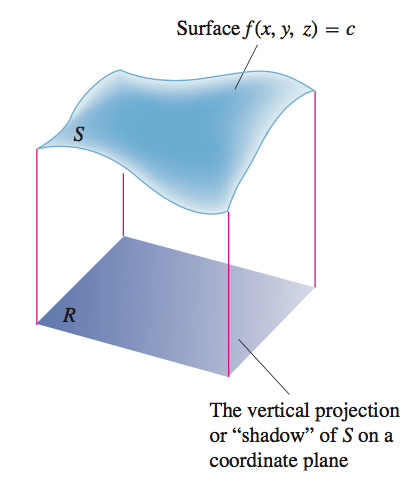
\includegraphics[width=0.6\textwidth]{surface0.png}
    \caption{As we soon see, the integral of a function $g(x,y,z)$ 
    over a surface $S$ in space can be calculated by evaluating 
    a related double integral over the vertical projection or "shadow"
    of $S$ on a coordinate plane.}
    \label{fig:fig2}
\end{figure}
\begin{figure}[htbp]
    \centering
    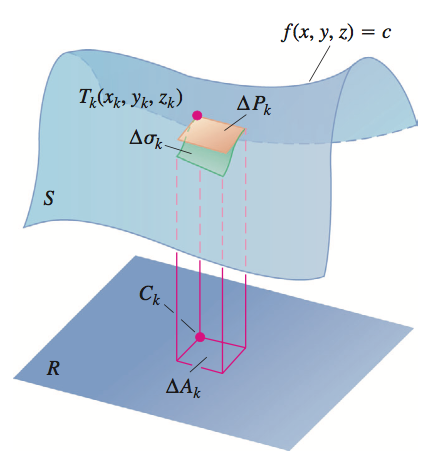
\includegraphics[width=0.6\textwidth]{surface1.png}
    \caption{A surface $S$ and its vertical projection onto a plane beneath 
    it. You can think of $R$ as the shadow of $S$ on the plane. The tangent 
    plane $\Delta P_k$  approximates the surface patch $\Delta \sigma_k$  above $\Delta A_k.$}
    \label{fig:fig3}
\end{figure}

\subsection{Surface Area}
Figure~\ref{fig:fig3} shows a surface $S$ lying above its "shadow"
region $R$ in a plane beneath it. The surface is defined by the 
equation $f(x,y,z) = c$. If the surface is smooth ($\nabla f$ is continuous 
and never vanishes on $S$). We can define and calculate it area as a 
double integral over $R$.

\begin{figure}[htbp]
    \centering
    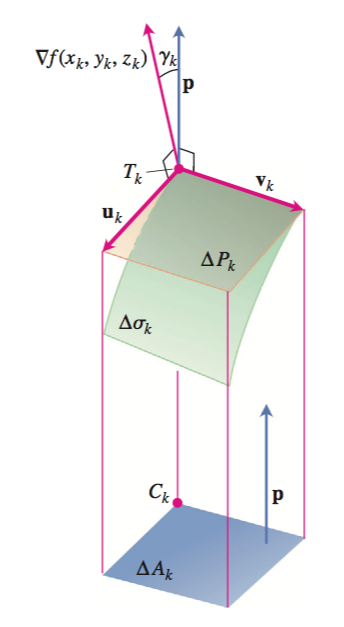
\includegraphics[height=0.8\textwidth, width=0.5\textwidth]{surface2.png}
    \caption{Magnified view from the preceding figure. The vector 
    $\bm{u}_k \times \bm{v}_k$  is parallel to the vector $\nabla f$ 
    because both vectors are normal to the plane of $\Delta P_k$.} 
    \label{fig:fig4}
\end{figure}

The first step in defining the area of $S$ is to partition the region 
$R$ into small rectangles $\Delta A_k$ of the kind we would use if we were 
defining an integral over $R$. Directly above each $\Delta A_k$ lies a patch 
of surface $\Delta \sigma_k$ that we may approximate by a parallelogram $\Delta P_k$
in the tangent plane to $S$ at a point $T_k(x_k,y_k,z_k)$ in $\Delta \sigma_k$.

Figure~\ref{fig:fig4} give a magnified view of $\Delta \sigma_k$ and $\Delta P_k$, showing the 
gradient vector $\nabla f_k$ at $T_k$ and a unit vector $\bm{p}$ that is 
normal to $R$. The figure also shows the angle $\gamma_k$ between $\nabla f_k$
and $\bm{p}$. In our case, this translates into the statement 
\[
    \left|\left(\bm{u}_k \times \bm{v}_k\right)\cdot\bm{p}\right| = \Delta A_k
\]
or 
\[
    \Delta P_k \left|\cos \gamma_k \right| = \Delta A_k
\]
or 
\[
    \Delta P_k = \frac{\Delta A_k}{\left|\cos \gamma_k \right|}
\]
We will have $\cos \gamma_k \ne 0$ is $\nabla f$ is not parallel to the ground plane 
and $\nabla f \cdot \bm{p} \ne 0$.

Since the patches $\Delta P_k $ approximates the surface patches $\Delta \sigma_k$
that fit together to make $S$, the sum 
\begin{equation}
    \sum \Delta P_k = \sum \frac{\Delta A_k}{\left|\cos \gamma_k\right|}
    \label{eq:eq6}
\end{equation}
If we refined the partition of $R$. In fact, the sums on the right-hand 
side of the equation~\ref{eq:eq6} are approximating sums for the 
double integral.
\begin{equation}
    \iint_R \frac{1}{\left|\cos \gamma \right|}\, \mathrm{d}A.
    \label{eq:eq7}
\end{equation}
We therefore define the area of $S$ to be the value of this integral 
whenever it exists. For any surface $f(x,y,z) = c$, we have $\displaystyle
\left|\nabla f \cdot \bm{p}\right| = \left|\nabla f\right| \left|\bm{p}\right|
\left|\cos \gamma\right|$, so
\[
    \frac{1}{\left|\cos \gamma\right|} = \frac{\left|\nabla f\right|}{\left|\nabla f \cdot \bm{p}\right|}.
\]
The area of the surface $f(x,y,z) = c$ over a closed and bounded plane 
region $R$ is 
\begin{equation}
    S = \iint_R \frac{\left|\nabla f\right|}{\left|\nabla f \cdot \bm{p}\right|}
       \,\mathrm{d}A.
    \label{eq:eq8}
\end{equation}

\begin{example}
    Find the area of the surface cut from the bottom of the paraboloid 
    $x^2 + y^2 -z =0$ by the plane $z=4$.
\end{example}

We have 
\[
    \begin{split}
        &f(x,y,z) = x^2 + y^2 - z,
    \nabla f = 2x\bm{i} + 2y\bm{j}  - \bm{k},\\
        &\left|\nabla f \cdot \bm{p} \right| = \left|\nabla f \cdot \bm{k}\right| = 1.\\
        & S = \iint_R \frac{\left|\nabla f \right|}{\left|\nabla f \cdot \bm{p}\right |}\, \mathrm{d}x\mathrm{d}y
            = \iint_{x^2 + y^2 \le 4} \sqrt{4x^2 + 4y^2 + 1}\,\mathrm{d}x\mathrm{d}y.
    \end{split}
    \]
\begin{example}
    Find the area of the cap cut from the hemisphere $x^2 + y^2 +z^2 = 2$, 
    by the cylinder $x^2 + y^2 \le 1$ in the xy-plane.
\end{example}

\subsection{Surface Integrals}
Suppose, for example, that we have an electrical charge distributed 
over a surface $f(x,y,z) = c$ like the one shown if Figure~\ref{fig:fig3}
and that the function $g(x,y,z)$ gives the charge per unit area (charge 
density) at each point on $S$. The we may calculate the total charge on 
$S$ as an integral of below:
\[
    \mathrm{Total charge} \approx \sum g(x_k, y_k, z_k)\Delta P_k = \sum g(x_k, y_k, z_k) 
    \frac{\Delta A_k}{\left|\cos \gamma \right|}
    \]
If $f$, the function defining the surface $S$, and its first derivatives 
are continuous, and if $g$ is continuous over $S$, then the sums on the 
right-hand side of the last equation approach the limit
\begin{equation}
    \iint_R g(x,y,z)\frac{\mathrm{d}A}{\left|\cos \gamma \right|}
    = \iint_R g(x,y,z) \frac{\left|\nabla f \right|}{\left|\nabla f \cdot \bm{p}\right |}\,\mathrm{d}A.
    \label{eq:eq10}
\end{equation}

\textbf{The Surface Area Differential and the Differential Form for Surface Integrals}
\[
    \bm{d}\sigma  = \frac{\left|\nabla f\right|}{\left|\nabla f \cdot \bm{p} \right|}
    \]
\[
    \iint_S g \, \mathrm{d}\sigma
    \]

\begin{example}
    Integrate $g(x,y,z)=xyz$ over the surface of the cube cut from 
    the first octant by the planes $x = 1, y = 1, z = 1$
    (Figure ~\ref{fig:fig5})
\end{example}
\begin{figure}[htbp]
    \centering
    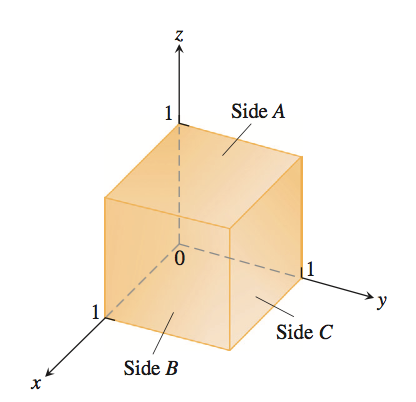
\includegraphics[height=0.6\textwidth, width=0.6\textwidth]{surface3.png}
    \caption{The cube in example above.}
    \label{fig:fig5}
\end{figure}

\subsection{Orientation}
We call a smooth surface $S$ \textbf{orientable} or \textbf{two-sided} if it is possible to 
define a field $\bm{n}$ of unit normal vectors on $S$ that varies 
continuously with position. Once $\bm{n}$ has been chosen, we say 
that we have \textbf{oriented } the surface, and we call the surface together 
with its normal field an \textbf{oriented surface}. The vector $\bm{n}$ 
at any point is called the \textbf{positive direction} at that point.
\begin{figure}[htbp]
    \centering
    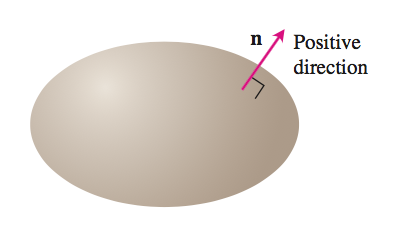
\includegraphics[height=0.5\textwidth, width=0.6\textwidth]{surface4.png}
    \caption{Smooth closed surface in space is orientable. The outward unit normal
    vector defines the positive direction at each point.}
    \label{fig:fig6}
\end{figure}
\begin{figure}[htbp]
    \centering
    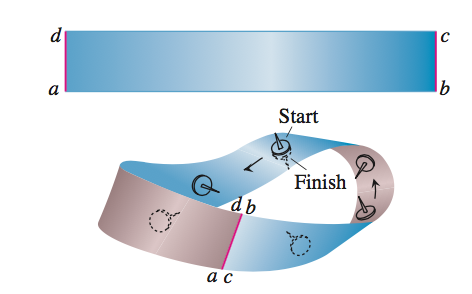
\includegraphics[height=0.5\textwidth, width=0.7\textwidth]{surface5.png}
    \caption{The Mobius band is a non-orientable or one-side surface.}
    \label{fig:fig7}
\end{figure}
\subsection{Surface Integral for Flux}
Suppose that $\bm{F}$ is a continuous vector field defined over an 
oriented surface $S$ and that $\bm{n}$ is the chosen unit normal 
field on the surface. We call the integral of $\bm{F}\cdot\bm{n}$ 
over $S$ the flux of $\bm{F}$ across $S$ in the positive direction.
\begin{definition}
    The \textbf{flux} of a three-dimensional vector field $\bm{F}$ across 
    an oriented surface $S$ in the direction of $\bm{n}$ is 
    \[
        Flux = \iint_S \bm{F}\cdot \bm{n}\, \mathrm{d}\sigma
    \]
\end{definition}

The definition is analogous to the flux of a two-dimensional field 
$\bm{F}$ across a plane curve $C$. In the plane, the flux is 
\[
    \int_C \bm{F}\cdot\bm{n}\,\mathrm{d}s,
\]
the integral of the scalar component of $\bm{F}$ normal to the curve.

If $\bm{F}$ is the velocity field of a three-dimensional fluid flow,
the flux of $\bm{F}$ across surface $S$ is the net rate at which 
fluid is crossing $S$ in the chosen positive direction. If $S$ is part 
of a surface $g(x,y,z) = c$, then $\bm{n}$ may be taken to be one of 
the two fields 
\begin{equation}
    \bm{n} = \pm\frac{\nabla g}{\left|\nabla g \right|}
    \label{eq:eq11}
\end{equation}
depending on which one gives the preferred direction. The corresponding 
flux is 
\begin{equation}
    \begin{split}
        \textrm{Flux} & = \iint_S \bm{F}\cdot\bm{n}\, \mathrm{d}\sigma\\
        \\
        & = \iint_S \left(\bm{F}\cdot\frac{\pm\nabla g}{\left|\nabla g\right|}\right)
            \frac{\left|\nabla g\right|}{\left|\nabla g\cdot\bm{p}\right|}\,\mathrm{d}A\\ \\
        & = \iint_S \bm{F}\cdot\frac{\nabla g}{\left|\nabla g\cdot\bm{p}\right|}\,\mathrm{d}A
    \end{split}
\end{equation}

\begin{example}
    Find the flux of $\bm{F} = yz\bm{j} + z^2\bm{k}$ outward through the 
    surface $S$ cut from the cylinder $y^2 + z^2 = 1, z \ge 0$ by the plane 
    $x = 0$ and $x = 1$. See Figure~\ref{fig:fig6}.
\end{example}
\begin{figure}[htbp]
    \centering 
    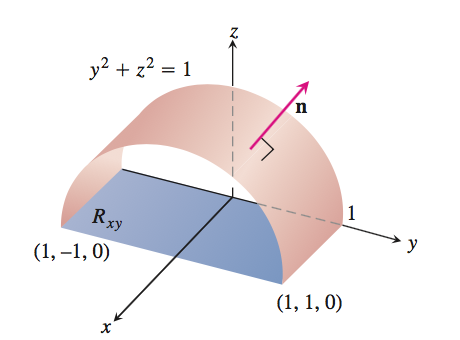
\includegraphics[height=0.5\textwidth, width=0.5\textwidth]{surface6.png}
    \caption{Calculating the flux of a vector field outward through
    this surface. The area of the shadow region $R_{xy}$ is 2.}
    \label{fig:fig8}
\end{figure}
\TheSolution The outward normal field on $S$ may be calculated from 
the gradient of $g(x,y,z) = y^2 + z^2$ to be 
\[
    \bm{n} = +\frac{\nabla g}{\left| \nabla g\right|} = 
    \frac{2y\bm{j} + 2z\bm{k}}{\sqrt{4y^2 + 4z^2}} = \frac{2y\bm{j}+2z\bm{k}}{2}
     = y\bm{j} + z\bm{k}.
    \]
With $\bm{p} = \bm{k}$, we also have 
\[
    \mathrm{d}\sigma = \frac{\left|\nabla g\right|}{\left|\nabla g \cdot \bm{k} \right|}
    \mathrm{d}A = \frac{2}{\left|2z\right|}\mathrm{d}A = \frac{1}{z}\mathrm{d}A.
    \]
\[
    \bm{F}\cdot \bm{n} = \left(yz\bm{j} + z^2\bm{k}\right) \cdot \left(y\bm{j} + z\bm{k}\right)
     = z\left(y^2 + z^2\right) = z.
    \]

\[
    \iint_S \bm{F} \cdot \bm{n} \, \mathrm{d}\sigma  = \iint_S z \frac{1}{z}\,\mathrm{d}A 
     = \iint_{R_{xy}} \, \mathrm{d}A = 2.
    \]

\subsection{Parametrized Surfaces}
We have defined curves in the plane in three different ways:

Explicit form: $y = f(x)$,

Implicit form: $F(x,y) = 0$,

Parametric vector form: $\bm{r}(t) = f(t)\bm{i} + g(t)\bm{j}$.

We have analogous definition of surface in space:

Explicit form: $z = f(x,y)$,

Implicit form: $F(x,y,z) = 0$.

There is also a parametric form that gives the position 
of a point on the surface as a vector function of two 
variables. The present section extends the investigation 
of surface area and surface integrals to surface described 
parametrically.

\subsubsection{Parametrizations of Surfaces}

Let 
\begin{equation}
    \bm{r}(u,v) = f(u,v)\bm{i} + g(u,v)\bm{j} + h(u,v)\bm{k}
    \label{eq:eq12}
\end{equation}
be a continuous vector function that is defined on a region $R$
in the $uv$-plane.

\begin{example}
    Find a parametrization of the cone
    \[
        z = \sqrt{x^2+y^2}, 0 \le z \le 1.
    \]
\end{example}

\begin{example}
    Find a parametrization of the sphere 
    \[
        x^2 + y^2 +z^2 = a^2
    \]
\end{example}

\begin{example}
    Find a parametrization of the cylinder 
    \[
        x^2 + \left(y-3\right)^2 = 9, 0 \le z \le 5.
    \]
\end{example}

\subsubsection{Surface Area}
For details see \textbf{section 1.2.1}.
\subsubsection{Surface Integral}
For detail see \textbf{section 1.3}
\subsubsection{Flux}
\begin{example}
    Find the flux of $\bm{F} = yz\bm{i} + x\bm{j} -z^2\bm{k}$
    outward through the parabolic cylinder $y = x^2$, 
    $0 \le x \le x, 0 \le z \le 4$.
\end{example}

\section{Path Independence, Potential Functions, and Conservative 
Fields}

In gravitational and electric fields, the amount of work 
it takes to move a mass or a charge from one point to 
another depends only on the object's initial and final 
positions and not on the path taken in between.

\subsection{Path Independence}
If $A$ and $B$ are two points in an open region $D$ in space, 
the work $\int\bm{F}\cdot\mathrm{d}\bm{r}$ done in moving a 
particle from $A$ to $B$ by a field $\bm{F}$ defined on $D$ 
usually depends on the path taken. For some special 
field, however, the integral's value is the same for all
paths from $A$ to $B$.

\begin{definition}
    Let $\bm{F}$ be a field defined on an open region $D$ in 
    space, and suppose that for any two points $A$ and $B$
    the work $\int_A^B \bm{F} \cdot \mathrm{d}\bm{r}$ done in 
    moving from $A$ to $B$ is the same over all paths from
    $A$ to $B$. Then the integral $\bm{F} \cdot \mathrm{d}\bm{r}$
    is path independent in $D$ and the field $\bm{F}$ is 
    conservative on $D$.
\end{definition}

Under differentiability conditions normally met in practice,
a field $\bm{F}$ is conservative if and only if it is 
the gradient of a scalar function, that is, if and only 
if $\bm{F} = \nabla f$ for some $f$. The function $f$ 
is called the potential function.

\begin{definition}
    If $\bm{F}$ is a field defined on $D$ and $\bm{F} = \nabla f$
    for some scalar function $f$ on $D$, then $f$ is called 
    a \textbf{potential function for $\bm{F}.$}
\end{definition}
\subsection{Line Integrals in Conservative Fields}
\begin{theorem}{\rm \textbf{The Fundamental Theorem of Line Integral}}\\
    Let $\bm{F} = M\bm{i} + N\bm{j} + P\bm{k}$ be a vector 
    field whose component are continuous throughout an 
    open connected $D$ in space. Then there exists a 
    differentiable function $f$ such that 
    \[
        \bm{F} = \nabla f = \frac{\partial f}{\partial x}\bm{i} + 
        \frac{\partial f}{\partial y}\bm{j} + \frac{\partial f}{\partial z}
        \bm{k}
    \]
    if and only if for all points $A$ and $B$ in $D$ the
    value of $\int_A ^B\bm{F} \cdot \mathrm{d}\bm{r}$
    is independent of the path joining $A$ to $B$ in $D$.

    If the integral is independent of the path from
    $A$ to $B$, its value is 
    \[
        \int_A^B\bm{F} \cdot \mathrm{d}\bm{r} = f(B) - f(A).
    \]
\end{theorem}
\begin{example}
    Find the work done by the conservative field 
    \[
        \bm{F} = yz\bm{i} + xz\bm{j} + xy\bm{k}
    \]
along any smooth curve $C$ joining the point $A(-1,3,9)$ to $B(1,6,-4)$.
\end{example}

\begin{theorem}{\rm \textbf{Closed-Loop Property of Conservative Fields}}
    The following statements are equivalent.
    \begin{enumerate}
        \item $\int \bm{F} \cdot \mathrm{d}\bm{r} = 0$ around every closed loop in $D$.
        \item The field $\bm{F}$ is conservative on $D$.
    \end{enumerate}
\end{theorem}

\subsection{Find Potentials for Conservative Fields}
\begin{theorem}
    Suppose that the domain of $\bm{F}$ is connected and simply connected.
    Let Let $\bm{F} = M\bm{i} + N\bm{j} + P\bm{k}$ be a vector 
    field whose component have continuous first partial derivatives. Then,
    $\bm{F}$ is conservative if and only if 
    \[
        \frac{\partial P}{\partial y} = \frac{\partial N}{\partial z}, 
        \frac{\partial M}{\partial z} = \frac{\partial P}{\partial x}, 
        \frac{\partial N}{\partial x} = \frac{\partial M}{\partial y}, 
        \]
\end{theorem}

\begin{example}
    Show that $\bm{F} = (e^x\cos y + yz)\bm{i} + (xz - e^x\sin y)\bm{j} 
    + (yz + z)\bm{k}$ is conservative and find a potential function for it.
\end{example}

\section{Green's Theorem in the Plane}
In this section we consider how to evaluate the integral if it is not 
associated with a conservative vector field, but is a flow or flux 
integral across a closed curve in the xy-plane.

\subsection{Divergence}
We need new ideas for Green's theorem. The first is the idea of the 
divergence of a vector field at a point, sometimes called the flux 
density of the vector field by physicists and engineers. 

Suppose that $\bm{F}(x,y) = M(x,y)\bm{i} + N(x,y)\bm{j}$ is the velocity 
field of a fluid flow in the plane and that the first partial derivatives 
of $M$ and $N$ are continuous at each point of a region $R$. Let $(x,y)$ be a 
point in $R$ and let $A$ be a small rectangle with one corner at $(x,y)$ 
that, along with its interior, lies entirely in $R$. The sides of the 
rectangle parallel to the coordinate axes, have lengths of $\Delta x$ and $\Delta y$.
The rate at which fluid leaves the rectangle across the bottom edge is 
approximately, see Figure~\ref{fig:fig9}
\[
    \bm{F}(x,y) \cdot \bm{-j} \Delta x = -N(x,y)\Delta x
\]
\begin{figure}[htbp]
    \centering 
    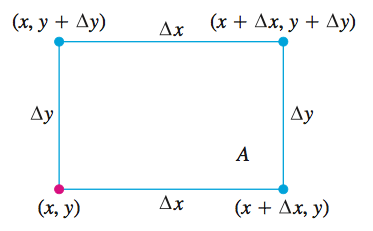
\includegraphics[height=0.3\textwidth, width=0.4\textwidth]{divergence1.png}
    \caption{The rectangle for defining the divergence (flux density) 
    of a vector field at point $(x,y)$.}
    \label{fig:fig9}
\end{figure}

Exit Rates:
\begin{enumerate}
    \item Top: $\bm{F}(x,y+\Delta y) \cdot \bm{j} \Delta x = N(x,y+\Delta y)\Delta x$
    \item Bottom:$\bm{F}(x,y) \cdot \bm{-j} \Delta x = -N(x,y)\Delta x$
    \item Right: $\bm{F}(x+\Delta x,y) \cdot \bm{i} \Delta y = M(x+\Delta x,y)\Delta y$
    \item Left: $\bm{F}(x,y) \cdot \bm{-i} \Delta y = -M(x,y)\Delta y.$
\end{enumerate}

Combining opposite pairs gives:
\[
    {\rm \textbf{Flux across rectangle boundary}} \approx \left(
    \frac{\partial M}{\partial x} + \frac{\partial N}{\partial y}\right)
    \Delta x \Delta y.
\]
We now divide by $\Delta x \Delta y$ to estimate the total flux per unit area of 
flux density for the rectangle:
\[
{\rm {div \bm{F}}} = \frac{\partial M}{\partial x} + \frac{\partial N}{\partial y}
\]

\begin{definition}
    The divergence (flux density) of a vector field $\bm{F} = M\bm{i} + N\bm{j}$ 
    at the point $(x,y)$ is 
    \[
        {\rm div} \bm{F} = \frac{\partial M}{\partial x} + \frac{\partial N}{\partial y}
    \]
\end{definition}
\begin{example}
    Find the divergence of $\bm{F}(x,y) = (x^2 - y)\bm{i} + (xy - y^2)\bm{j}$.
\end{example}

\subsection{Spin Around an Axis: The k-Component of Curl}
The second idea we need for Green's theorem has to do with measuring how 
a paddle wheel spins at a point in a fluid flowing in a plane region. This 
idea gives some sense of how the fluid is circulating around axes located 
at different points and perpendicular to the region. Physicists sometimes 
refer to this as the circulation density of a vector field $\bm{F}$ at a point.
To obtain it, we return to the velocity field.
\[
    \bm{F}(x,y) = M(x,y)\bm{i} + N(x,y)\bm{j} 
\]
and the rectangle $A$. The rectangle is redrawn here as Figure~\ref{fig:fig10}.
\begin{figure}[htbp]
    \centering 
    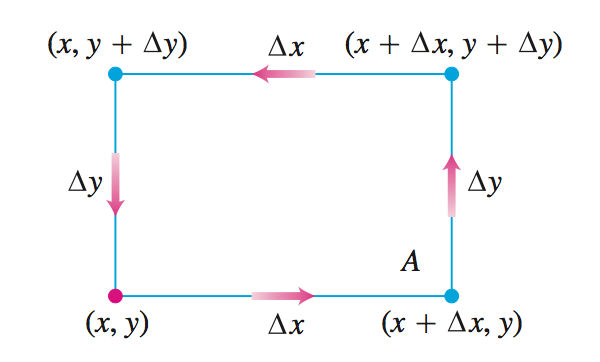
\includegraphics[height=0.3\textwidth, width=0.5\textwidth]{curl1.png}
    \caption{The rectangle for defining the curl (circulation density) 
    of a vector field at point $(x,y)$.}
    \label{fig:fig10}
\end{figure}

The counterclockwise circulation of the velocity $\bm{F}$ around the boundary 
of $A$ is the sum of flow rates along the sides.
\begin{enumerate}
    \item Top: $\bm{F}(x,y+\Delta y) \cdot \bm{-i} \Delta x = -M(x,y+\Delta y)\Delta x$
    \item Bottom:$\bm{F}(x,y) \cdot \bm{i} \Delta x = M(x,y)\Delta x$
    \item Right: $\bm{F}(x+\Delta x,y) \cdot \bm{j} \Delta y = N(x+\Delta x,y)\Delta y$
    \item Left: $\bm{F}(x,y) \cdot \bm{-j} \Delta y = -N(x,y)\Delta y.$
\end{enumerate}

We add opposite pairs to get:
\[
    {\rm \textbf{Circulation along the boundary}} \approx 
    \left(\frac{\partial N}{\partial x} - \frac{\partial M}{\partial y}\right)
    \Delta x\Delta y.
\]
\begin{definition}
    The k-component of the curl (circulation density) of a vector field 
    $\bm{F} = M\bm{i} + N\bm{j}$ at the point $(x,y)$ is the scalar 
    \[
        {\rm curl}\bm{F} \cdot \bm{k} = 
    \frac{\partial N}{\partial x} - \frac{\partial M}{\partial y}
\]
\end{definition}

\begin{example}
    Find the k-component of the curl for the vector field 
    \[
        \bm{F}(x,y) = (x^2 - y)\bm{i} + (xy - y^2)\bm{j}
    \]
\end{example}

\subsection{Two Forms for Green's Theorem}
In one form, Green's Theorem says that under suitable conditions the 
outward flux of a vector field across a simple closed curve in the 
plane equals the double integral of the divergence of the field 
over the region enclosed by the curve.
\begin{theorem}{\rm \textbf{Flux-Divergence or Normal Form}}\\
    The outward flux of a field $\bm{F} = M\bm{i}+N\bm{j}$ across a 
    simple closed curve $C$ equals the double integral of div $\bm{F}$
    over the region $R$ enclosed by $C$.
    \begin{equation}
        \oint_C\bm{F} \cdot \bm{n}\,\mathrm{d}s = 
        \oint_C M\,\mathrm{d}y - N\,\mathrm{d}x = 
        \iint_R \left(\frac{\partial M}{\partial x} + \frac{\partial N}{\partial y}\right)\,
        \mathrm{d}x\mathrm{d}y
        \label{eq:eq13}
    \end{equation}
\end{theorem}

In another form, Green's Theorem says that the counterclockwise circulation 
of a vector around a simple closed curve is the double integral of the 
k-component of the curl of the field over the region enclosed by the curve.

\begin{theorem}{\rm \textbf{(Circulation-Curl or Tangential Form)}}
    The counterclockwise circulation of a field $\bm{F} = M\bm{i}+N\bm{j}$
    around a simple closed curve $C$ in the plane equals the double integral 
    of $\left({\rm curl}\bm{F} \right) \cdot \bm{k}$ over the region $R$ enclosed 
    by $C$.
    \begin{equation}
        \oint_C \bm{F} \cdot \bm{T}\,\mathrm{d}s = \oint_C M\,\mathrm{d}x 
        + N\,\mathrm{d}y = \iint_R \left(\frac{\partial N}{\partial x} - \frac{\partial M}{\partial y}\right)
        \, \mathrm{d}x\mathrm{d}y.
        \label{eq:eq14}
    \end{equation}
\end{theorem}

\begin{example}
    Verify both forms of Green's Theorem for the field 
    \[
        \bm{F}(x,y) = (x-y)\bm{i} + x\bm{j}
    \]
    and the region $R$ bounded by the unit circle 
    \[
        C: \bm{r}(t) = \cos t\bm{i} + \sin t\bm{j}, 0 \le t \le 2\pi.
    \]
\end{example}
\begin{example}
    Evaluate the integral 
    \[
        \oint_C xy\,\mathrm{d}y - y^2\,\mathrm{d}x
    \]
    where $C$ is the square cut from the first quadrant by the lines 
    $x = 1$ and $y = 1$.
\end{example}

\begin{example}
    Calculate the outward flux of the field $\bm{F}(x,y) = x\bm{i} + y^2\bm{j}$
    across the square bounded by the lines $x = \pm 1$ and $y = \pm 1$.
\end{example}

\begin{example}
    Verify the circulation form of Green's Theorem on the annular ring 
    $R:h^2 \le x^2 + y^2 \le 1, 0 < h < 1$, if 
    \[
        M = \frac{-y}{x^2+y^2}, N = \frac{x}{x^2 + y^2}
    \]
    Here $R$ is not simply connected.
\end{example}

\section{The Divergence Theorem and a Unified Theory}
The divergence form of Green's Theorem in the plane states that 
the net outward flux of the field across a simple closed curve 
can be calculated by integrating the divergence of the field over 
the region enclosed by the curve. The corresponding theorem 
in three dimensions, called the Divergence Theorem, states that
the net outward flux of a vector field across a closed surface in 
space can be calculated by integrating the divergence of the field 
over the region enclosed by the surface.

\subsection{Divergence in Three dimension}
The divergence of a vector field $\bm{F} = M(x,y,z)\bm{i} + N(x,y,z)\bm{j}
+ P(x,y,z)\bm{k}$ is the scalar function 
\[
    {\rm div} \bm{F} = \nabla\cdot\bm{F} = \frac{\partial M}{\partial x} 
    + \frac{\partial N}{\partial y} + \frac{\partial P}{\partial z}.
\]
\begin{example}
    Find the divergence of $\bm{F} = 2xz\bm{i} - xy\bm{j} -z \bm{k}$.
\end{example}

\subsection{The Gauss-Ostrogradskii Formula}
\begin{theorem}
    Let $\mathbb{R}^3$ be three-dimensional space with a fixed coordinates 
    system $x,y,z$ and $\overline{D}$ a compact domain in $\mathbb{R}^3$ 
    bounded by piecewise-smooth surface. Let $P, Q, R$ be smooth functions 
    in the closed domain $\overline{D}$. Then the following relation holds:
    \[
        \begin{split}
        \iiint_{\overline{D}} \left(\frac{\partial P}{\partial x} + \frac{\partial Q}{\partial y}
        + \frac{\partial R}{\partial z}\right)\,\mathrm{d}x\mathrm{d}y\mathrm{d}z \\
            = \iint_{\partial \overline{D}} P dy\wedge dz + Qdz\wedge dx + R dx \wedge dy.
        \end{split}
    \]
\end{theorem}

If we denote $\bm{F} = (P, Q, R)$, the Gauss-Ostrogradskii theorem can be 
written as \[
    \iiint_{\overline{D}} \nabla \cdot \bm{F}\, dV = \iint_{\partial \overline{D}} 
    \bm{F} \cdot \bm{n} d\sigma.
\]
\begin{example}
    Find the flux of $\bm{F} = xy\bm{i}+yz\bm{j}+xz\bm{k}$ outward 
    through the surface of the cube cut from the first octant 
    by the plane $x = 1, y = 1, z = 1.$
\end{example}

\begin{example}
    Find the net outward flux of the field 
    \[
        \bm{F} = \frac{x\bm{i} + y\bm{j} + z\bm{k}}{\rho^3} ,
        \rho = \sqrt{x^2 + y^2 + z^2}
        \]
    across the boundary of the region: $D: 0<a^2\le x^2+y^2+z^2\le b^2$
\end{example}

\subsection{Gauss's Law: One of the Four Great Laws of Electromagnetic 
Theory}
The outward flux of $\bm{E}$ across any sphere centered at the origin 
is $\frac{q}{\epsilon_0}$, and the result is not confined to spheres. In electro-
magnetic theory, the electric field created by a point charge $q$ located 
at the origin is 
\[
    \bm{E}(x,y,z) = \frac{1}{4\pi\epsilon_0}\frac{q}{|\bm{r}|^2}\frac{r}{|r|} 
     = \frac{q}{4\pi\epsilon_0}\frac{x\bm{i}+y\bm{j}+z\bm{k}}{\rho^3}
     \]
Gauss's law:
\[
    \iint_S \bm{E}\cdot\bm{n}d\sigma = \frac{q}{\epsilon_0}
\]
\section{Stokes' Theorem}
In three dimensional, the circulation around a point $P$ in a plane is 
described with a vector. This vector is normal to the plane of the 
circulation and points in the direction that gives it a right-hand 
relation to the circulation line. The length of the vector gives the
rate of the fluid's rotation, which usually varies as the circulation 
plane is tilted about $P$. It turns out that the vector of greatest circulation 
in a flow with velocity field $\bm{F} = M\bm{i} + N\bm{j} + P\bm{k}$
is the curl vector
\begin{equation}
    {\rm curl}\bm{F} = \left(\frac{\partial P}{\partial y} - \frac{\partial N}{\partial z}\right)
    \bm{i} + \left(\frac{\partial M}{\partial z} - \frac{\partial P}{\partial x}\right)\bm{j}
    + \left(\frac{\partial N}{\partial x} - \frac{\partial M}{\partial y}\right)\bm{k}.
\end{equation}

If we denote 
\begin{equation}
    \nabla = \bm{i}\frac{\partial}{\partial x} + \bm{j}\frac{\partial}{\partial y} + \bm{k}\frac{\partial}{\partial z}.
\end{equation}
The curl of $\bm{F}$ is $\nabla \times \bm{F}$:
\[
    \begin{split}
        \nabla \times \bm{F} & = \left| \begin{array}{ccc} \bm{i} & \bm{j} & \bm{k} \\
        \frac{\partial}{\partial x} & \frac{\partial}{\partial y} & \frac{\partial}{\partial z}\\
    M & N & P \end{array} \right|\\
        & = \left(\frac{\partial P}{\partial y} - \frac{\partial N}{\partial z}\right)
    \bm{i} + \left(\frac{\partial M}{\partial z} - \frac{\partial P}{\partial x}\right)\bm{j}
    + \left(\frac{\partial N}{\partial x} - \frac{\partial M}{\partial y}\right)\bm{k}\\
        & = {\rm curl }\bm{F}.
    \end{split}
\]

\begin{example}
    Find the curl of $\bm{F} = \left(x^2 - y\right)\bm{i} + 4z\bm{j} + x^2\bm{k}.$
\end{example}

\begin{example}
    For a 1-form 
    \[
        \omega = P\mathrm{d}x + Q\mathrm{d}y + R\mathrm{d}z
    \]
    defined in a domain $D$ in $\mathbb{R}^3$ we obtian
    \[
        \mathrm{d}\omega = \left(\frac{\partial R}{\partial y} 
        - \frac{\partial Q}{\partial z}\right)\mathrm{d}y \wedge \mathrm{d}z
        +\left(\frac{\partial P}{\partial z} - \frac{\partial R}{\partial x}\right)
        \mathrm{d}z \wedge \mathrm{d}x 
        + \left(\frac{\partial Q}{\partial x} - \frac{\partial P}{\partial y}\right)\mathrm{d}x \wedge \mathrm{d}y
    \]
\end{example}

\begin{theorem}
    Let $S$ be an oriented piecewise-smooth compact two dimensional 
    surface with boundary $\partial S$ embedded in a domain $G \subset \mathbb{R}^3$,
    in which a smooth 1-form $\omega = P\mathrm{d}x + Q\mathrm{d}y +
    R\mathrm{d}z$ is defined. Then the following relation holds:
    \[
        \int_{\partial S}P\mathrm{d}x + Q\mathrm{d}y + R\mathrm{d}z
        = \iint_{S} \left(\frac{\partial R}{\partial y} 
        - \frac{\partial Q}{\partial z}\right)\mathrm{d}y \wedge \mathrm{d}z
        +\left(\frac{\partial P}{\partial z} - \frac{\partial R}{\partial x}\right)
        \mathrm{d}z \wedge \mathrm{d}x 
        + \left(\frac{\partial Q}{\partial x} - \frac{\partial P}{\partial y}\right)\mathrm{d}x \wedge \mathrm{d}y
    \]
    where the orientation of the boundary $\partial S$ is chosen consisting 
    with the orientation of the surface $S$.

    In other notation, this means that 
    \[
        \int_{S} \mathrm{d}\omega = \int_{\partial S} \omega.
    \]
\end{theorem}

\begin{figure}[htbp]
    \centering
    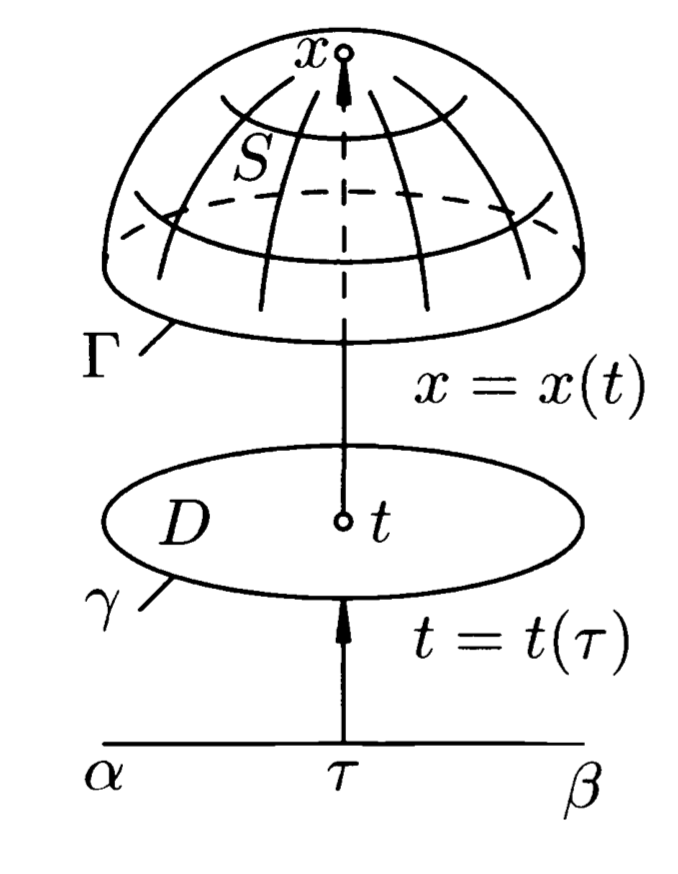
\includegraphics[width=0.5\textwidth]{stokes.png}
    \caption{Parameters of a surface for Stokes.}
    \label{fig:fig11}
\end{figure}
Let us show the proof of the Stokes theorem. To avoid expressions 
that are really too cumbersome, we shall write out only the first,
main part of its two expressions, and with some simplifications 
even in that. To be specific, let us introduce the notation 
$x^1, x^2, x^3$ for the coordinates of a point $x \in \mathbb{R}^3$
and verify only that 
\[
    \int_{\partial S} P(x)\mathrm{d}x^1 = \iint_S \frac{\partial P}{\partial x^2}\mathrm{d}x^2\wedge\mathrm{d}x^1
     + \frac{\partial P}{\partial x^3} \mathrm{d}x^3\wedge\mathrm{d}x^1
     \]

For simplicity we shall assume that $S$ can be obtained by a smooth 
mapping $x = x(t)$ of domain $D$ in the plane $\mathbb{R}^2$ of the 
variables $t^1, t^2$ and bounded by a smooth curve $\gamma = \partial D$
parametrized via a mapping $t = t(\tau)$ by the points of the closed 
interval $\alpha < \tau < \beta$ (See Figure~\ref{fig:fig11}). Then the boundary 
$\Gamma = \partial S$ of the surface $S$ can be written as $x = x(t(\tau))$,
where $\tau$ ranges over the closed inteval $[\alpha, \beta]$.
Using the definiton of the integral over a curve, Green's 
formula for a plane domain $D$, and the definiton of the integral 
over a parametrized surface, we find successively.
\[
    \begin{split}
        \int_{\Gamma}P(x)\,\mathrm{d}x^1& = \int_{\alpha}^{\beta}
        P\left(x(t(\tau))\right)\left(\frac{\partial x^1}{\partial t^1} \frac{\mathrm{d} t^1}{\mathrm{d}\tau} 
        + \frac{\partial x^1}{\partial t^2} \frac{\mathrm{d} t^2}{\mathrm{d}\tau}\right)
        \mathrm{d}\tau \\\\
        & = \int_{\gamma} P\left(x(t)\right)\left(\frac{\partial x^1}{\partial t^1} {\mathrm{d}t^1} 
        + \frac{\partial x^1}{\partial t^2}{\mathrm{d}t^2}\right)\\\\
        & = \iint_D \left[\frac{\partial}{\partial t^1}\left(P\frac{\partial x^1}{\partial t^2}\right)
        - \frac{\partial}{\partial t^2}\left(P\frac{\partial x^1}{\partial t^1}\right)\right]
        \,\mathrm{d}t^1 \wedge \mathrm{d}t^2\\\\
        & = \iint_D\left(\frac{\partial P}{\partial t^1}\frac{\partial x^1}{\partial t^2} - 
        \frac{\partial P}{\partial t^2}\frac{\partial x^1}{\partial t^1} \right)
        \,\mathrm{d}t^1 \wedge \mathrm{d}t^2\\\\
        & = \iint_D \sum_{i=1}^{3}\left(\frac{\partial P}{\partial x^i}\frac{\partial x^i}{\partial t^1}
        \frac{\partial x^1}{\partial t^2}- 
        \frac{\partial P}{\partial x^i}\frac{\partial x^i}{\partial t^2}
        \frac{\partial x^1}{\partial t^1}\right)
        \,\mathrm{d}t^1 \wedge \mathrm{d}t^2\\\\
        & = \iint_D \left(\frac{\partial P}{\partial x^2}\frac{\partial x^2}{\partial t^1} 
        + \frac{\partial P}{\partial x^3}\frac{\partial x^3}{\partial t^1}\right)\frac{\partial x^1}{\partial t^2}\\\\
        & -\left( \frac{\partial P}{\partial x^2}\frac{\partial x^2}{\partial t^2} 
        + \frac{\partial P}{\partial x^3}\frac{\partial x^3}{\partial t^2}\right)\frac{\partial x^1}{\partial t^1}
         \, \mathrm{d}{t^1}\wedge\mathrm{d}{t^2}\\\\
         & = \iint_D\left(\frac{\partial P}{\partial x^2}\left|
        \frac{\partial (x^2, x^1)}{\partial (t^1, t^2)}\right| + \frac{\partial P}{\partial x^3}
        \left|\frac{\partial (x^3, x^1)}{\partial (t^1, t^2)}\right| \right)
         \, \mathrm{d}{t^1}\wedge\mathrm{d}{t^2}\\\\
         & = \iint_S\left(\frac{\partial P}{\partial x^2}\mathrm{d}x^2
         \wedge \mathrm{d}x^1 + \frac{\partial P}{\partial x^3}
         \,\mathrm{d}x^3 \wedge \mathrm{d}x^1\right)
    \end{split}
\]
\end{CJK}
\end{document}
